HTTPS stands for Hypertext Transfer Protocol Secure.
HTTPS is an extension of the Hypertext Transfer Protocol.
It is used for secure communication over a computer network,
and is widely used on the Internet [\cite{lam2000secure, karayiannis2019implementing}].
In HTTPS, the communication protocol is encrypted using Transport Layer Security [\cite{turner2014transport}]
or, formerly, Secure Sockets Layer [\cite{weaver2006secure}].
The protocol is therefore also referred to as HTTP over TLS or HTTP over SSL\@.
The principal motivations for HTTPS are authentication of the accessed website, and protection of the privacy and integrity
of the exchanged data while in transit.
It protects against \textit{man-in-the-middle attacks}.
The bidirectional encryption of communications between a client and server protects the communications against
eavesdropping and tampering [\cite{mayer2016tlscompare, jiang2019physical}].
The authentication aspect of HTTPS requires a trusted third party to sign server-side digital certificates.
This was historically an expensive operation, which meant fully authenticated HTTPS connections were usually found only
on secured payment transaction services and other secured corporate information systems on the World Wide Web.
In 2016, a campaign by the Electronic Frontier Foundation with the support of web browser developers led to the protocol
becoming more prevalent [\cite{he2014shadowcrypt}].
HTTPS is now used more often by web users than the original non-secure HTTP, primarily to protect
page authenticity on all types of websites;
secure accounts;
and to keep user communications, identity, and web browsing private [\cite{rescorla2000rfc2818}].

\subsection{What is an SSL Certificate?}\label{subsec:what-is-an-ssl-certificate?}
SSL stands for Secure Sockets Layer and, in short, it's the standard technology for keeping an internet connection
secure and safeguarding any sensitive data that is being sent between two systems, preventing criminals from reading
and modifying any information transferred, including potential personal details.
The two systems can be a server and a client, for example, a shopping website and browser, or server to server,
for example, an application with personal identifiable information or with payroll information.
SSL certificates are what enable websites to move from HTTP to HTTPS, which is more secure.
An SSL certificate is a data file hosted in a website's origin server.
SSL certificates make SSL or TLS (Transport Layer Security) encryption possible, and they contain the website's
public key and the website's identity, along with related information.
Devices attempting to communicate with the origin server will reference this file to obtain the public key and verify
the server's identity.
The private key is kept secret and secure.
SSL certificates include:
\begin{itemize}
    \item The domain name that the certificate was issued for
    \item Which person, organization, or device it was issued to
    \item Which certificate authority issued it
    \item The certificate authority's digital signature
    \item Associated sub-domains
    \item Issue date of the certificate
    \item Expiration date of the certificate
    \item The public key (the private key is kept secret)
\end{itemize}
The public and private keys used for SSL are essentially long strings of characters used for encrypting and decrypting data.
Data encrypted with the public key can only be decrypted with the private key, and vice versa.
\begin{figure}[H]
    \centering
    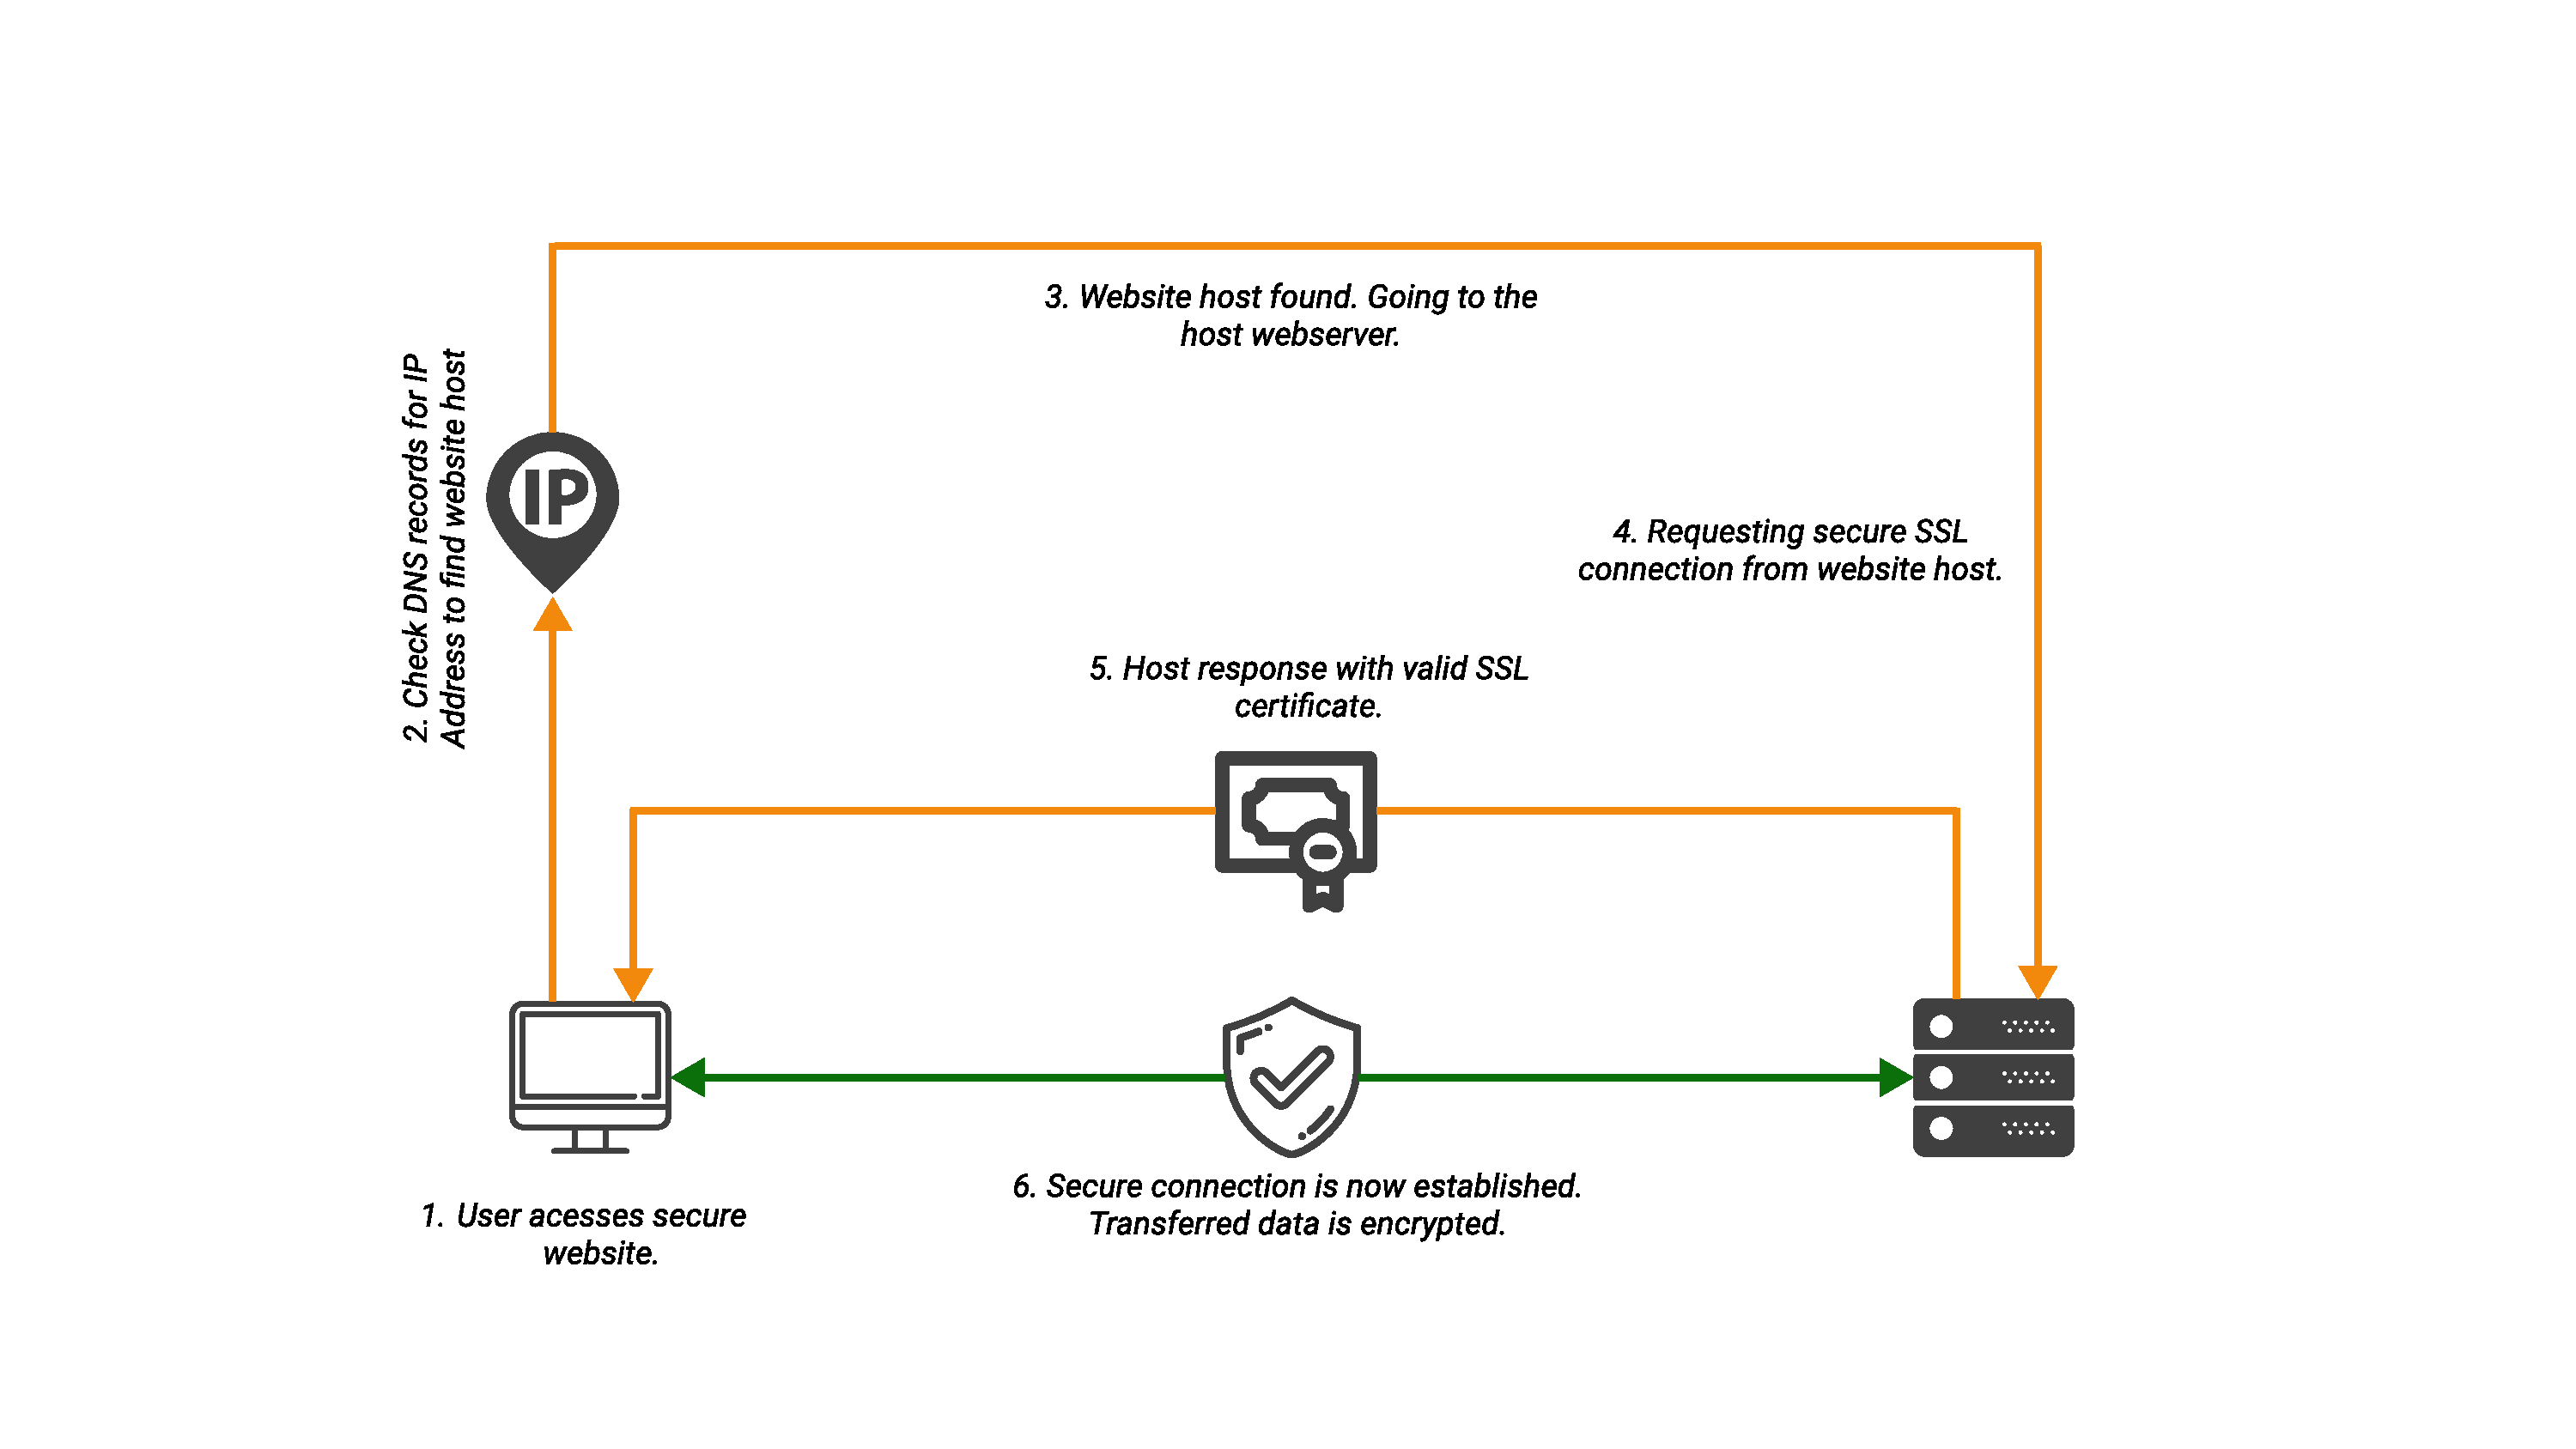
\includegraphics[width=1\textwidth]{Pictures/HTTPS_Flow}
    \caption{HTTPS flow diagram.}\label{fig:figure6}
\end{figure}

\subsection{Discussion on E2E Encryption}\label{subsec:discussion-on-e2e-encryption-over-https-protocol}
End-to-end encryption (E2EE) is a system of communication where only the communicating users can read the messages.
In principle, it prevents potential eavesdroppers -- including telecom providers, Internet providers,
and even the provider of the communication service -- from being able to access the cryptographic keys needed to
decrypt the conversation.
End-to-end encryption is intended to prevent data being read or secretly modified, other than by the true sender and
recipient.
The messages are encrypted by the sender but the third party does not have a means to decrypt them, and stores them
encrypted.
The recipients retrieve the encrypted data and decrypt it themselves.
Because no third parties can decipher the data being communicated or stored, for example, companies that provide
end-to-end encryption are unable to hand over texts of their customers' messages to the authorities.

It is important to note that E2EE does not equal privacy or security.
In many messaging systems, including email and many chat networks, messages pass through intermediaries and are stored
by a third party, from which they are retrieved by the recipient.
Even if the messages are encrypted, they are only encrypted 'in transit', and are thus accessible by the service provider,
regardless of whether server-side disk encryption is used.
Server-side disk encryption simply prevents unauthorized users from viewing this information.
It does not prevent the company itself from viewing the information, as they have the key and can simply decrypt this data.
This allows the third party to provide search and other features, or to scan for illegal and unacceptable content,
but also means they can be read and misused by anyone who has access to the stored messages on the third party system,
whether this is by design or via a backdoor.
This can be seen as a concern in many cases where privacy is very important, such as businesses whose reputation
depends on their ability to protect third party data, negotiations and communications that are important enough to
have a risk of targeted 'hacking' or surveillance, and where sensitive subjects such as health, and information about
minors are involved.
E2E encryption is to be implemented for mobile client.
In order to fulfill the E2E encryption topic, in ongoing section we discuss its successful implementation, the MTProto 2.0
protocol, of popular Telegram messenger.

\subsection{E2E Encryption in Telegram messenger}\label{subsec:e2e-encryption-in-telegram-messenger}
Telegram uses so-called MTProto 2.0 cryptographic protocol.
Before a message (or a multipart message) is transmitted over a network using a transport protocol, it is encrypted
in a certain way, and an external header is added at the top of the message that consists of a 64-bit key identifier
\textbf{auth\_key\_id} (that uniquely identifies an authorization key for the server as well as the user) and
a 128-bit message key \textbf{msg\_key}.
The authorization key \textbf{auth\_key} combined with the message key \textbf{msg\_key} define an actual 256-bit
key \textbf{aes\_key} and
a 256-bit initialization vector \textbf{aes\_iv}, which are used to encrypt the message using AES-256 encryption in
infinite garble extension (IGE) mode.
Note that the initial part of the message to be encrypted contains variable data
(session, message ID, sequence number, server salt) that obviously influences the message key and thus the AES key
and IV\@.
In MTProto 2.0, the message key is defined as the 128 middle bits of the SHA-256 of the message body
(including session, message ID, padding, etc.) prepended by 32 bytes taken from the authorization key.
In the older MTProto 1.0, the message key was computed as the lower 128 bits of SHA-1 of the message body,
excluding the padding bytes.
Where
\begin{itemize}
    \item \textbf{Authorization Key (auth\_key).} A 2048-bit key shared by the client device and the server,
    created upon user registration directly on the client device by exchanging Diffie-Hellman keys, and never
    transmitted over a network.
    Each authorization key is user-specific.
    There is nothing that prevents a user from having several keys that correspond to "permanent sessions"
    on different devices, and some of these may be locked forever in the event the device is lost.
    \item \textbf{Server Key.} A 2048-bit RSA key used by the server digitally to sign its own messages while
    registration is underway and the authorization key is being generated.
    The application has a built-in public server key which can be used to verify a signature but cannot be used
    to sign messages.
    A private server key is stored on the server and changed very infrequently.
    \item \textbf{Key Identifier (auth\_key\_id).} The 64 lower-order bits of the SHA1 hash of the authorization
    key are used to indicate which particular key was used to encrypt a message.
    Keys must be uniquely defined by the 64 lower-order bits of their SHA1, and in the event of a collision,
    an authorization key is regenerated.
    A zero key identifier means that encryption is not used which is permissible for a limited set of message types
    used during registration to generate an authorization key in a Diffie-Hellman exchange.
    For MTProto 2.0, SHA1 is still used here, because auth\_key\_id should identify the authorization key used
    independently of the protocol version.
    \item \textbf{Session.} A (random) 64-bit number generated by the client to distinguish between individual
    sessions (for example, between different instances of the application, created with the same authorization key).
    The session in conjunction with the key identifier corresponds to an application instance.
    The server can maintain session state.
    Under no circumstances can a message meant for one session be sent into a different session.
    The server may unilaterally forget any client sessions;
    clients should be able to handle this.
    \item \textbf{Server Salt.} A (random) 64-bit number changed every 30 minutes (separately for each session) at
    the request of the server.
    All subsequent messages must contain the new salt although, messages with the old salt are still accepted for
    a further 1800 seconds.
    Required to protect against replay attacks and certain tricks associated with adjusting the client clock to
    a moment in the distant future.
    \item \textbf{Message Identifier (msg\_id).} A (time-dependent) 64-bit number used uniquely to identify a
    message within a session.
    Client message identifiers are divisible by 4, server message identifiers modulo 4 yield 1 if the message is a
    response to a client message, and 3 otherwise.
    Client message identifiers must increase monotonically within a single session, the same as server message
    identifiers, and must approximately equal $unixtime \times 2^{32}$.
    This way, a message identifier points to the approximate moment in time the message was created.
    A message is rejected over 300 seconds after it is created or 30 seconds before it is created
    this is needed to protect from replay attacks.
    In this situation, it must be re-sent with a different identifier or placed in a container with a higher identifier.
    The identifier of a message container must be strictly greater than those of its nested messages.
\end{itemize}